\documentclass{article}

\usepackage{color}
\usepackage{graphicx}

\usepackage[cmex10]{amsmath}
\interdisplaylinepenalty=2500

\usepackage{amssymb}
\usepackage{amsthm}
\usepackage{mathtools}
\usepackage{float}
\usepackage{tikz}
\usepackage{epstopdf}
%\usepackage{natbib}
\usepackage{hyperref}

\graphicspath{ {figures/} }

\newtheorem{theorem}{Theorem}
\newtheorem{lemma}{Lemma}

\newcommand{\myeq}{=}
\newcommand{\expc}[1]{\mathrm{E} \! \left[#1\right]}
\newcommand{\re}[1]{\mathrm{Re}\! \left(#1\right)}
\newcommand{\im}[1]{\mathrm{Im}\! \left(#1\right)}
\newcommand{\prob}[1]{\mathrm{Pr}\! \left(#1\right)}
\newcommand{\probC}[1]{\mathrm{Pr}_\epsilon\! \left(#1\right)}

\newcommand{\saeed}[1]{{\color{red}[\textit{#1}]}}

%\newcommand{\saeed}[1]{}
\newcommand{\saeedlong}[1]{[\textit{#1}]}
%\newcommand{\saeedlong}[1]{}

\newcommand{\eqn}[1]{(\ref{#1})}

\newcommand{\fig}[1]{Fig.~\ref{#1}}

%\newcommand{\doc}[1]{{\tiny #1}}
\newcommand{\doc}[1]{}

\newcommand{\tikzfolder}{./tikz-files/}

\input{\tikzfolder tikz-styles}

%\usepackage{draftwatermark}
%\SetWatermarkText{DRAFT}
%\SetWatermarkScale{0.5}

\title{Alaleh's part regarding Spherical color mappings}
\date{\today}

\begin{document}
\maketitle

\saeed{Needs to be merged with Zihan's text about scalar color maps} There are two categories of color mapping methods:
\begin{itemize}
	\item Scalar Color Mapping: Consider a scalar value associated with each segment of a tract, which could  be FA or MD in this context. This type of color mappings provide a mapping from the chosen scalar quantity to a color. 
	\item Spherical Color Mapping: Unlike scalar color mapping, this type of mapping is usually from an inherent property of the tract segments to a color. A common choice is the orientation of the line segment. 
\end{itemize}

In this report, we examine 5 scalar and two spherical color mappings. The scalar color mappings are \saeed{Zihan's descriptions}. The spherical color mappings are 
\begin{itemize}
	\item Absolute value method [cite] is a commonly used color mapping which maps the major axes, i.e. \saeed{the anatomical names}, to major color components Red, Greed and Blue. The mapping is defined as \saeed{we need to choose the symbols and names}
	\begin{equation}
		f(\mathbf{s})=[|s_x|, \ |s_y|, \ |s_z|]^T
	\end{equation}
	where $\mathbf{s}=[s_x ,s_y, s_z]^T$ is the normalized vector corresponding to a line segment. 
	\begin{figure}
		\centering
		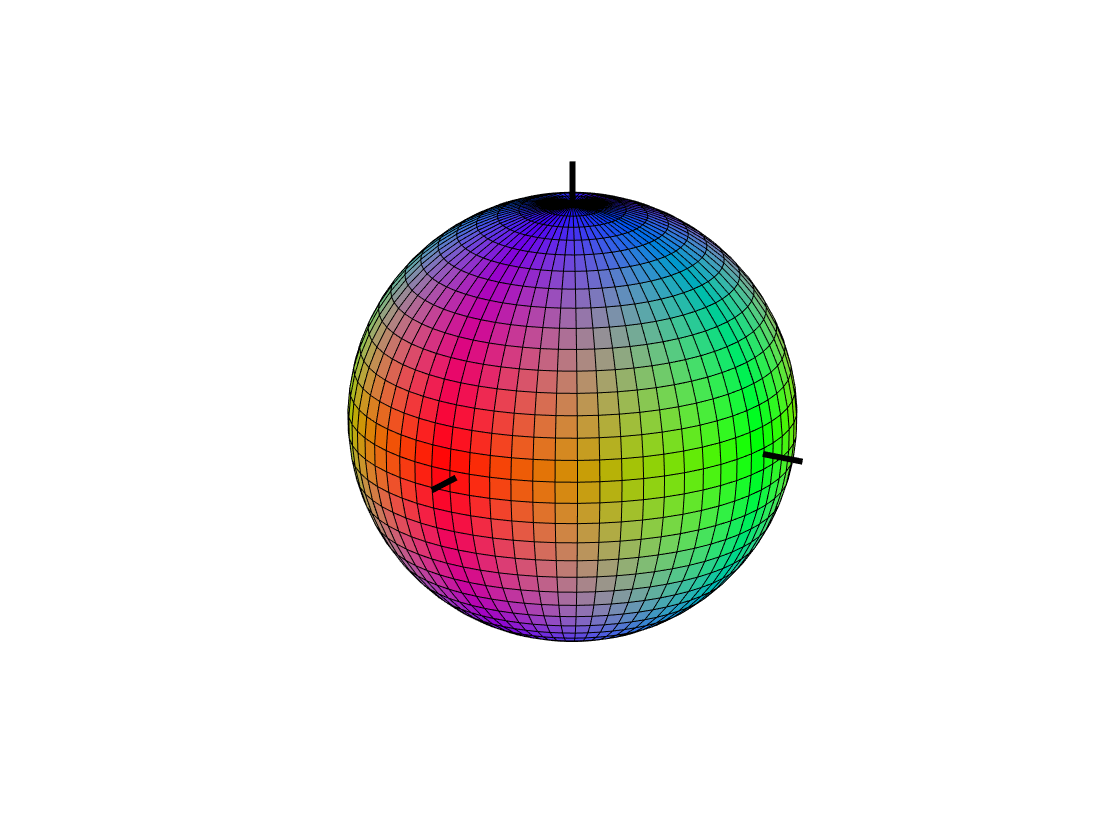
\includegraphics[width=0.35\textwidth]{absolute}
		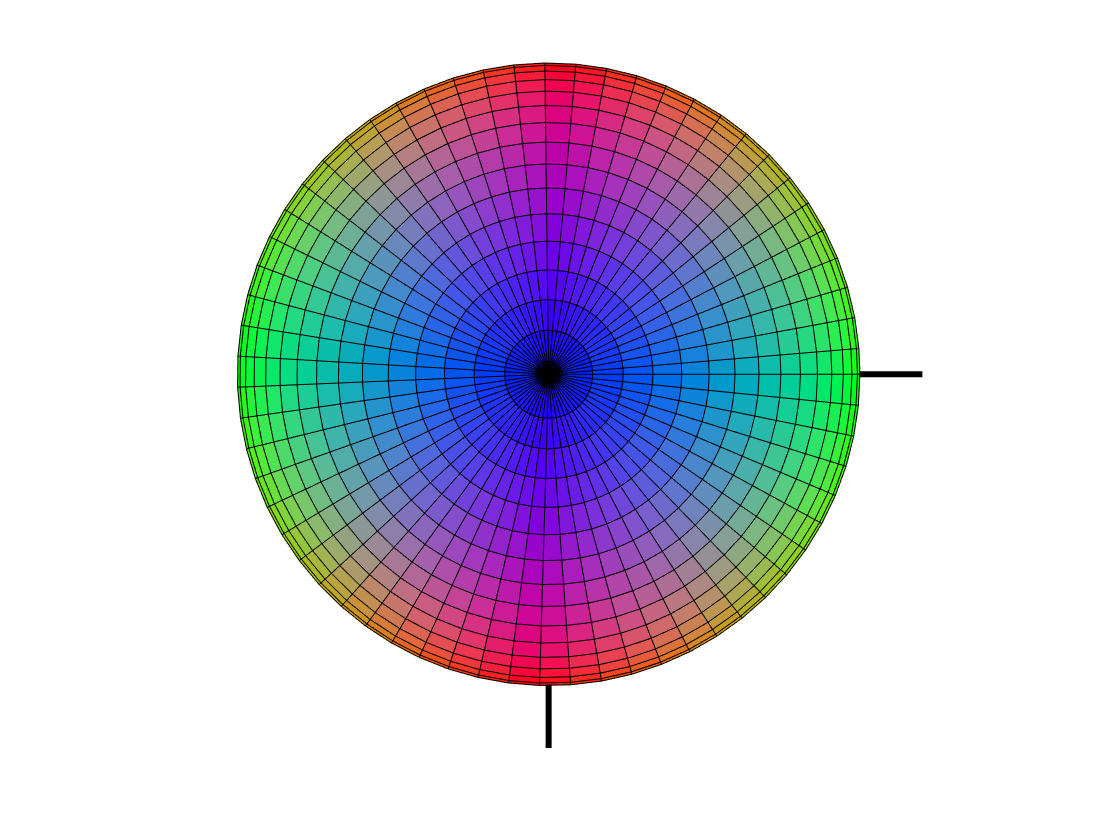
\includegraphics[width=0.3\textwidth]{absolute_top}
		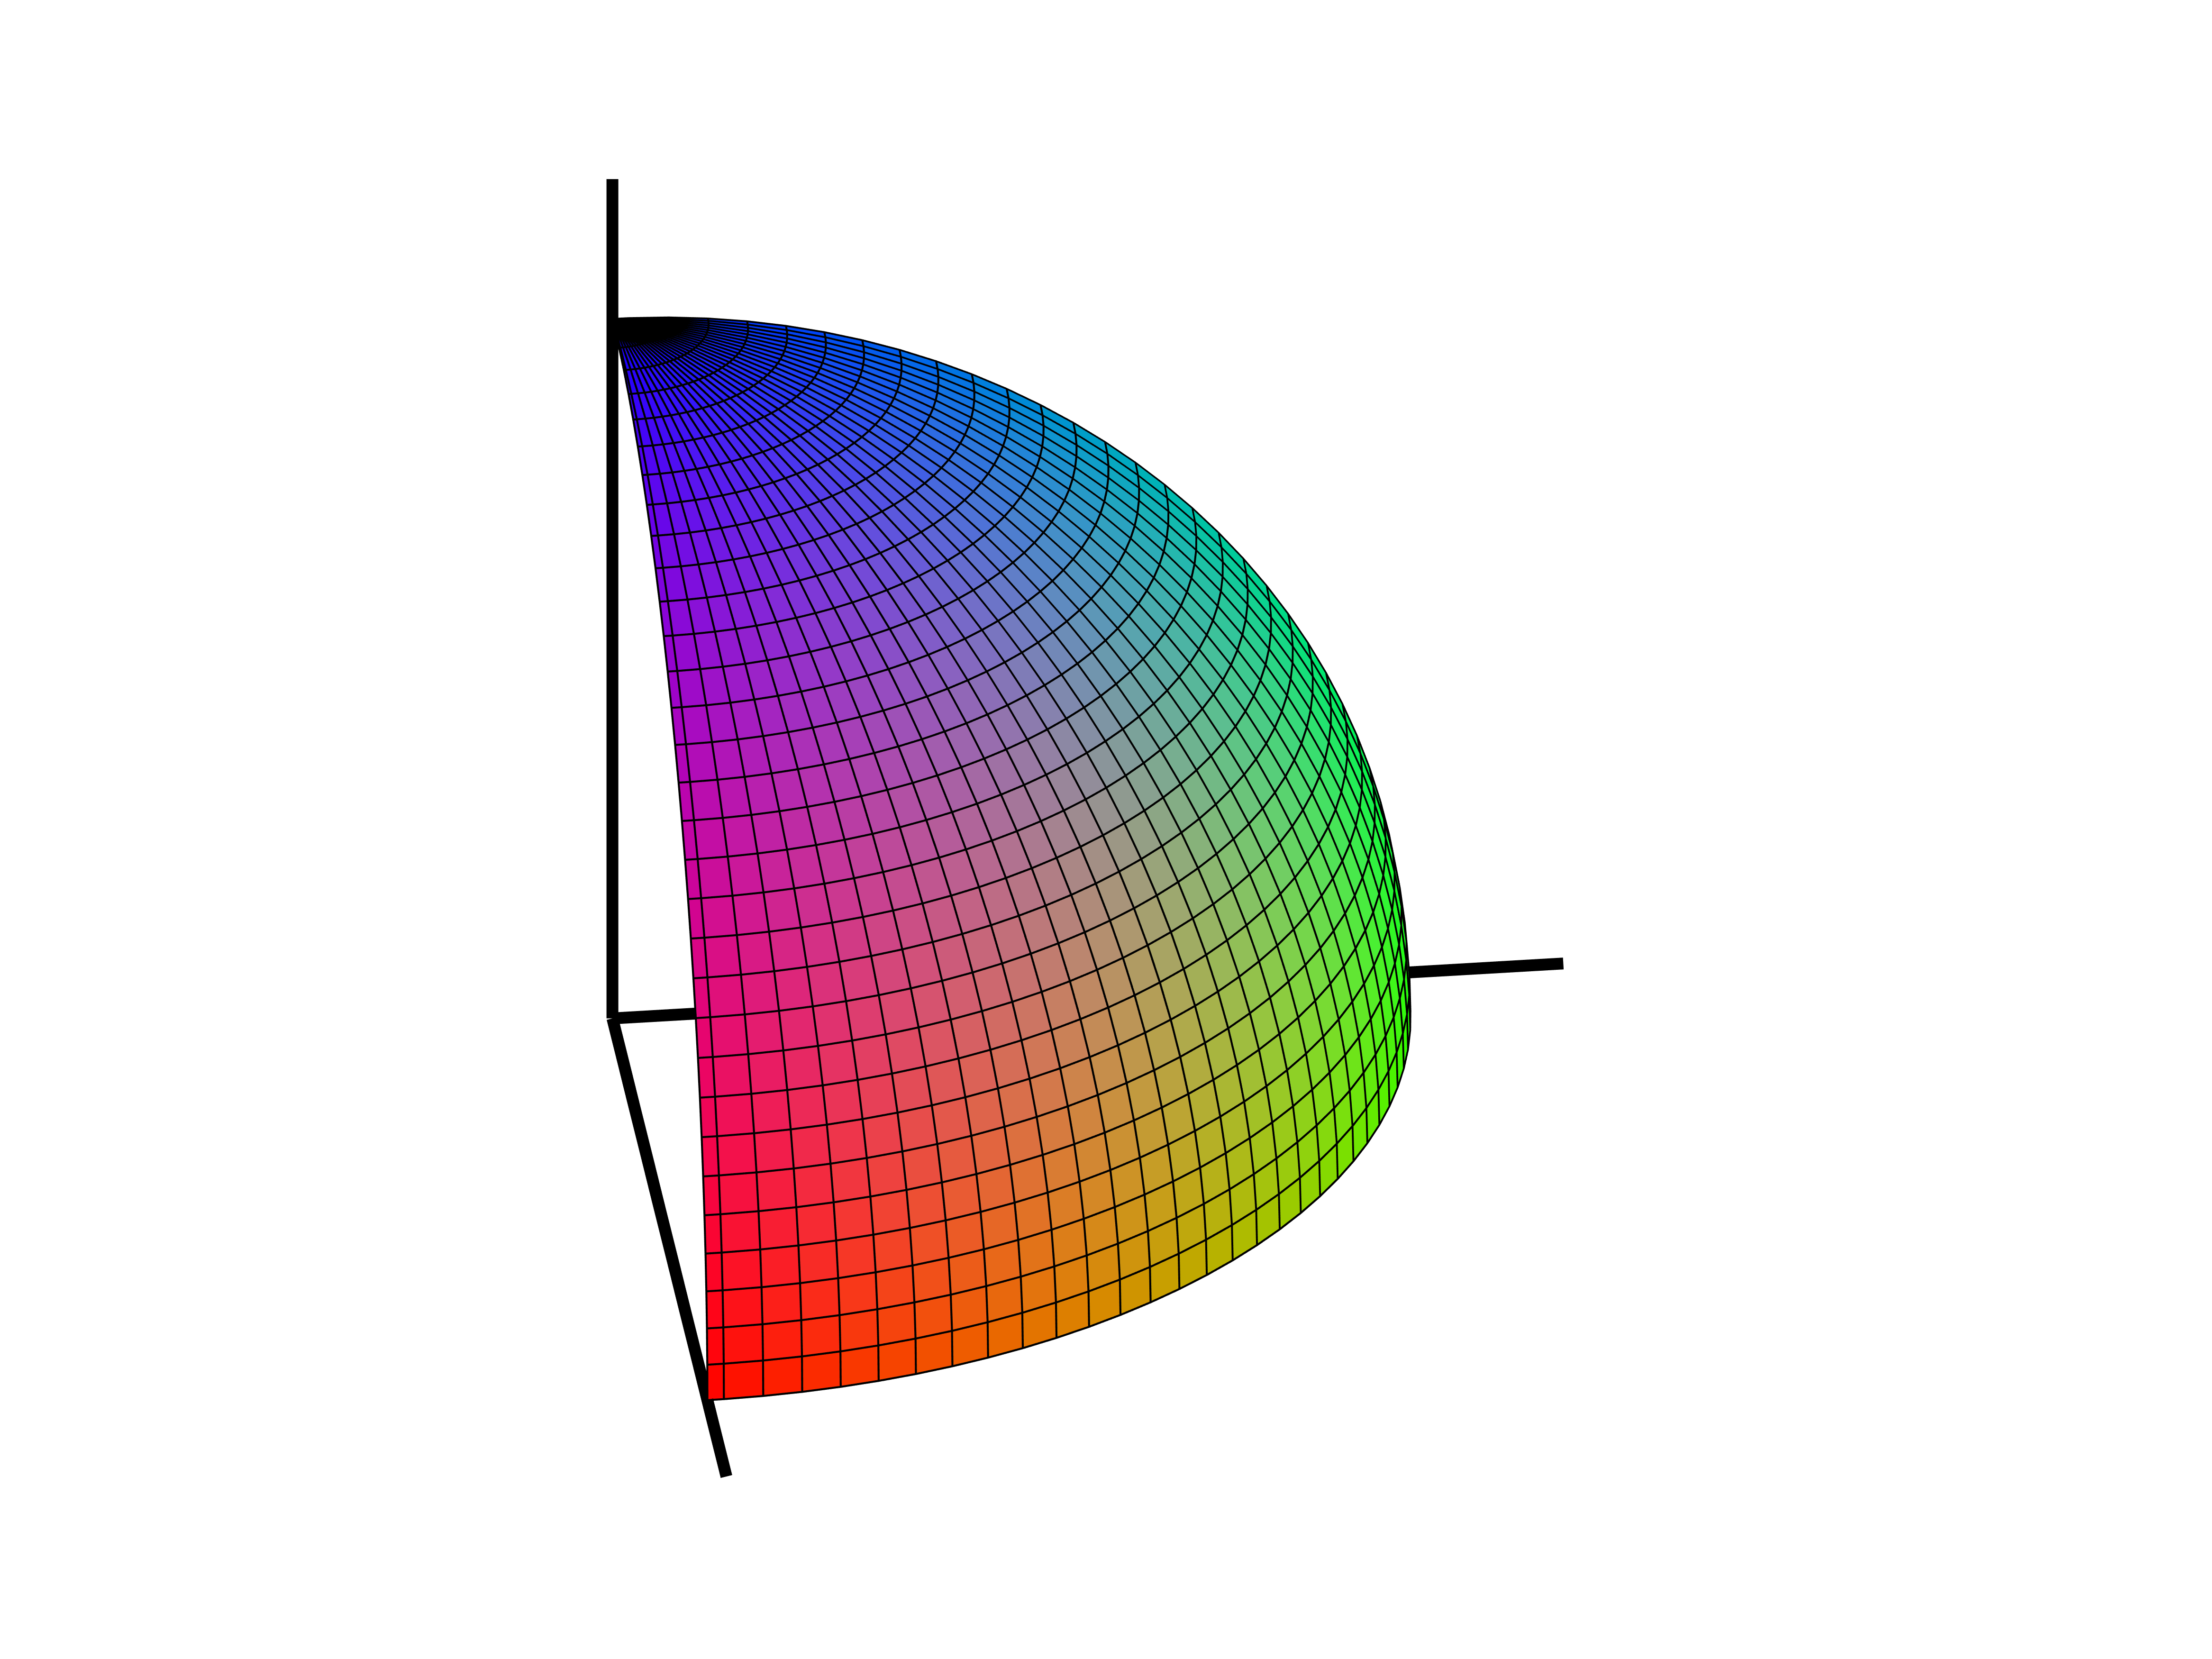
\includegraphics[width=0.3\textwidth]{absolute_octant}
		\caption{Absolute value method, colored sphere.}
	\end{figure}
	\item Boy's surface method [cite] \saeed{complete the name} is a more complicated color mapping scheme based on the immersion of Real Projective Plane in $\mathbb{R}^2$. The mapping is defined as 
	\begin{equation}
		f(\mathbf{s})=[f_1(\mathbf{s}), f_2(\mathbf{s}), f_3(\mathbf{s})]^T
	\end{equation}
	where 
	\begin{equation}
		f_i(\mathbf{s})=\sum_{j=0}^{\infty} c_{i,j} h_j(\mathbf{s}).
	\end{equation}
	The functions $h_j$ are the spherical harmonics, a similar concept to harmonics in Fourier analysis. As suggested by the authors in [cite], the summation is replaced with a partial sum to obtain a continuous mapping and the coefficients $c_{i,j}$ are adjusted manually for better results. 
\end{itemize}

	\begin{figure}
		\centering
		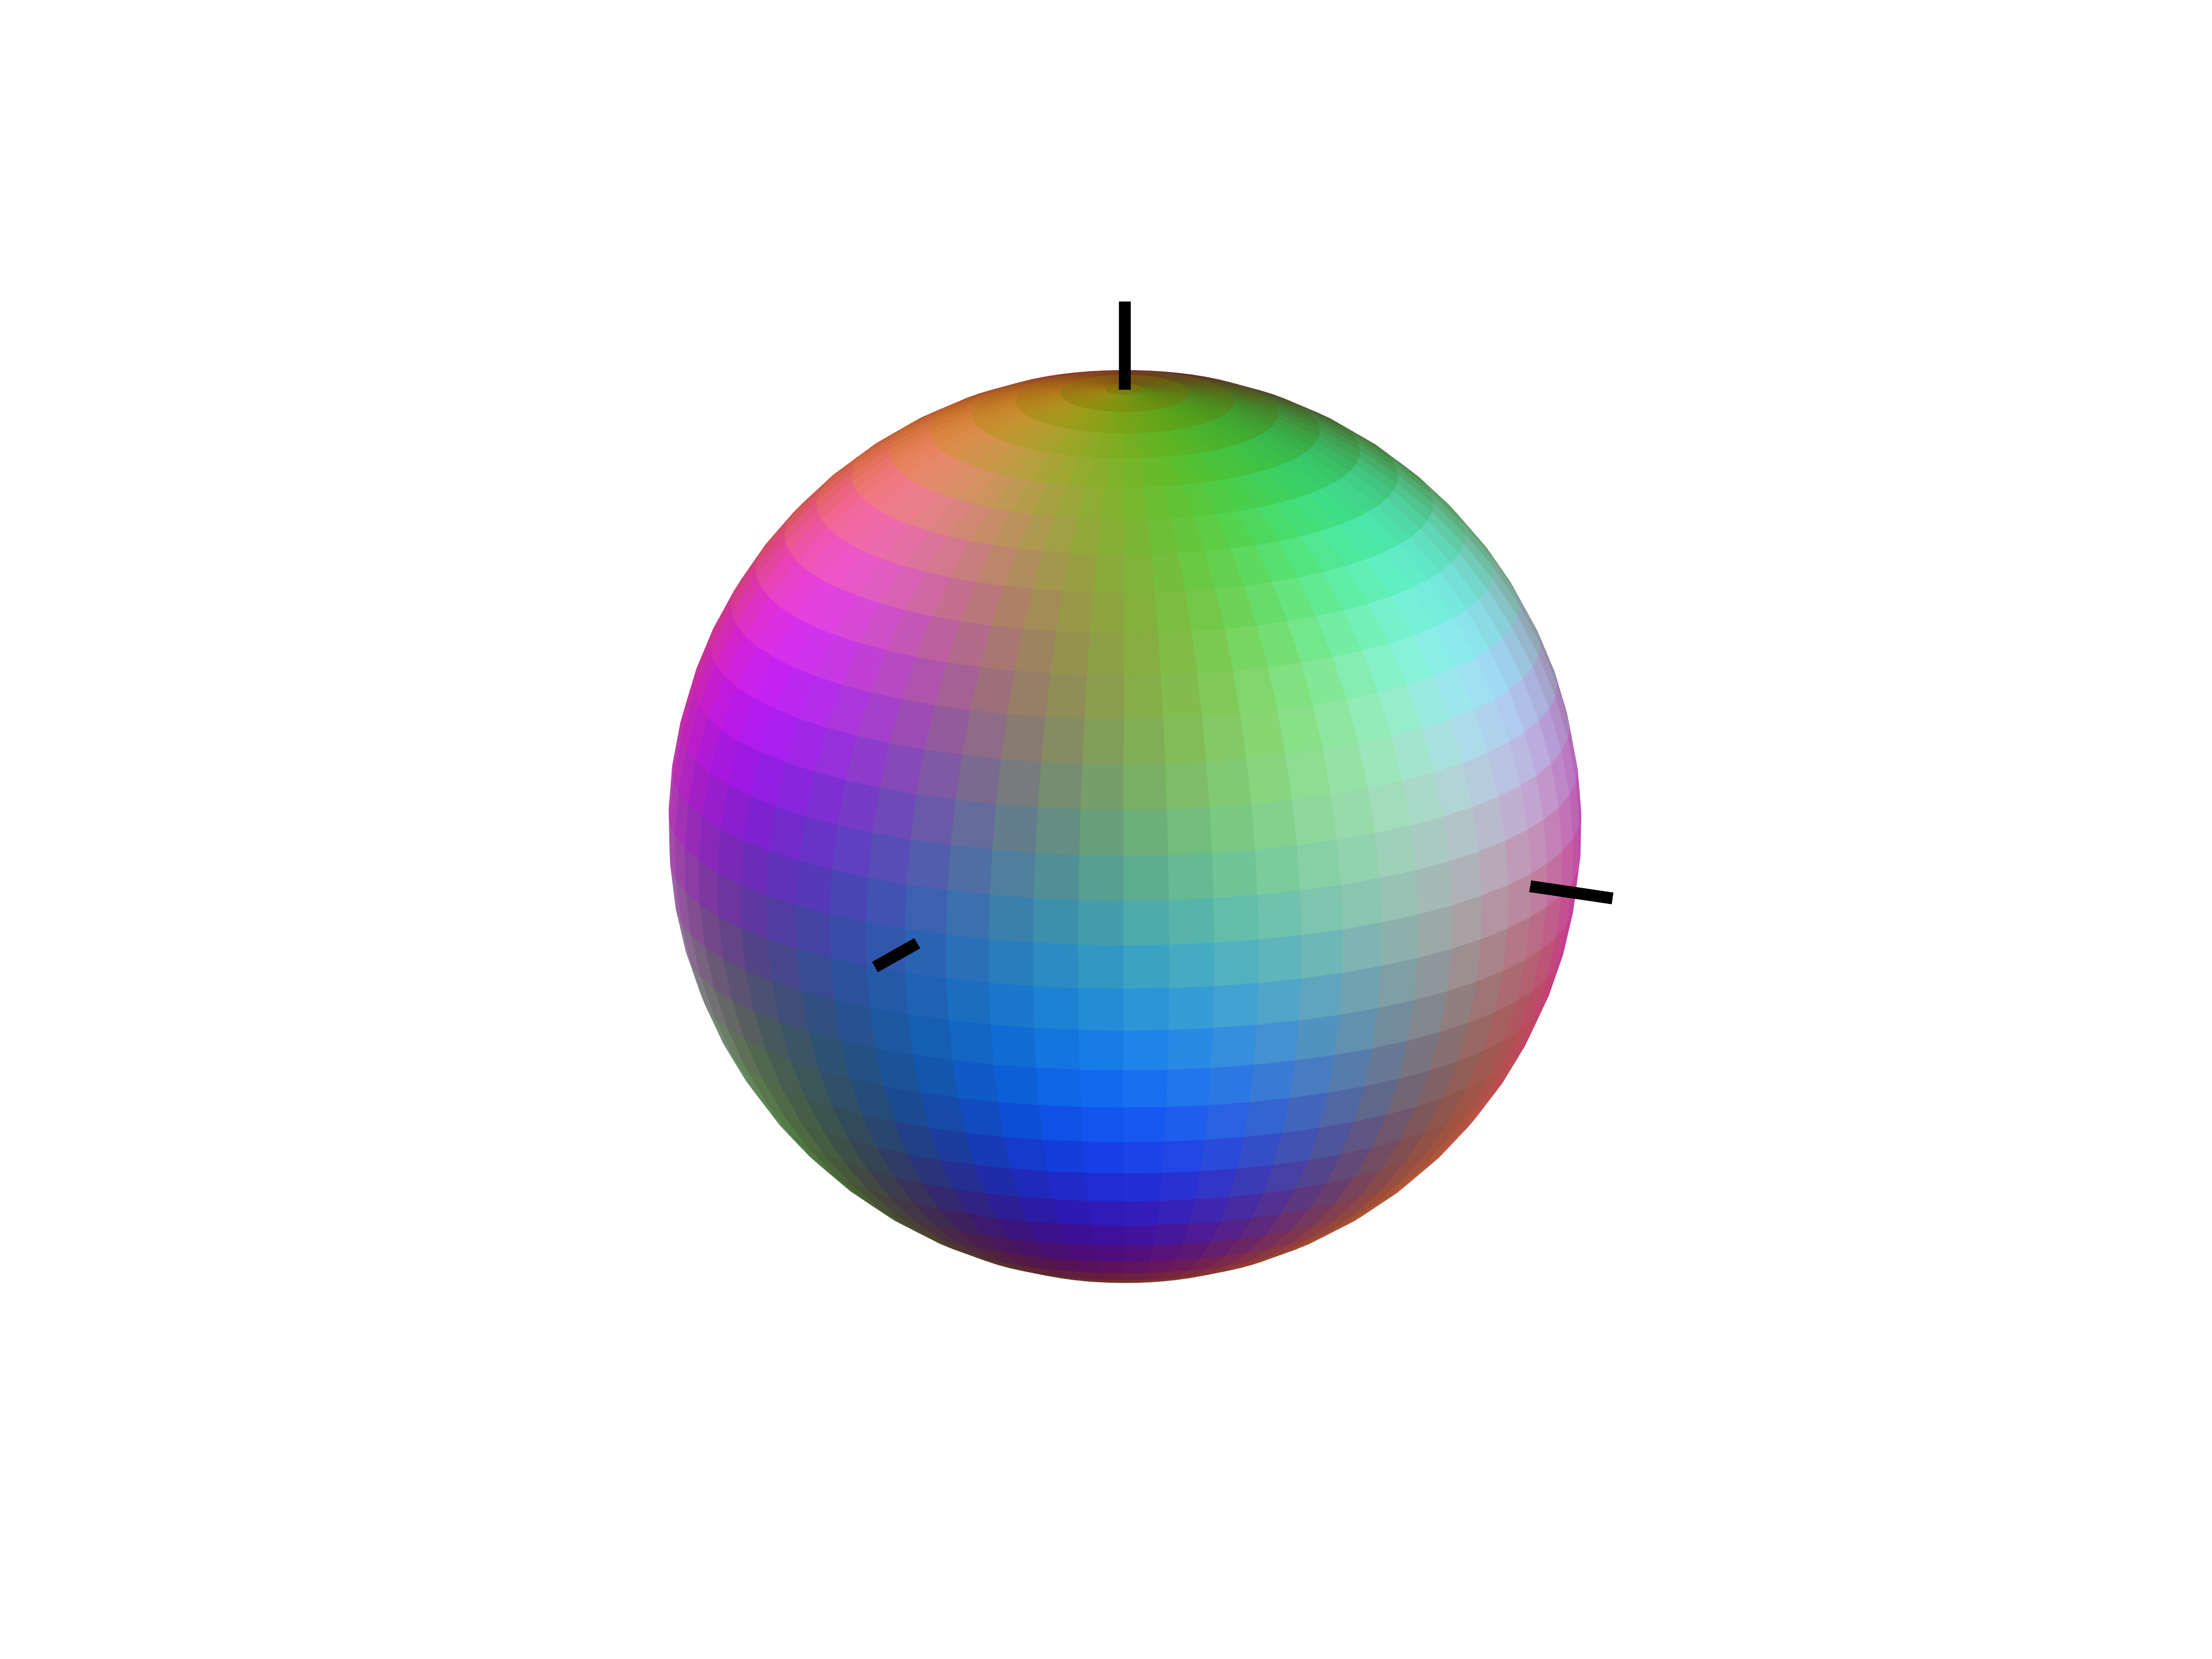
\includegraphics[width=0.33\textwidth]{boys}
		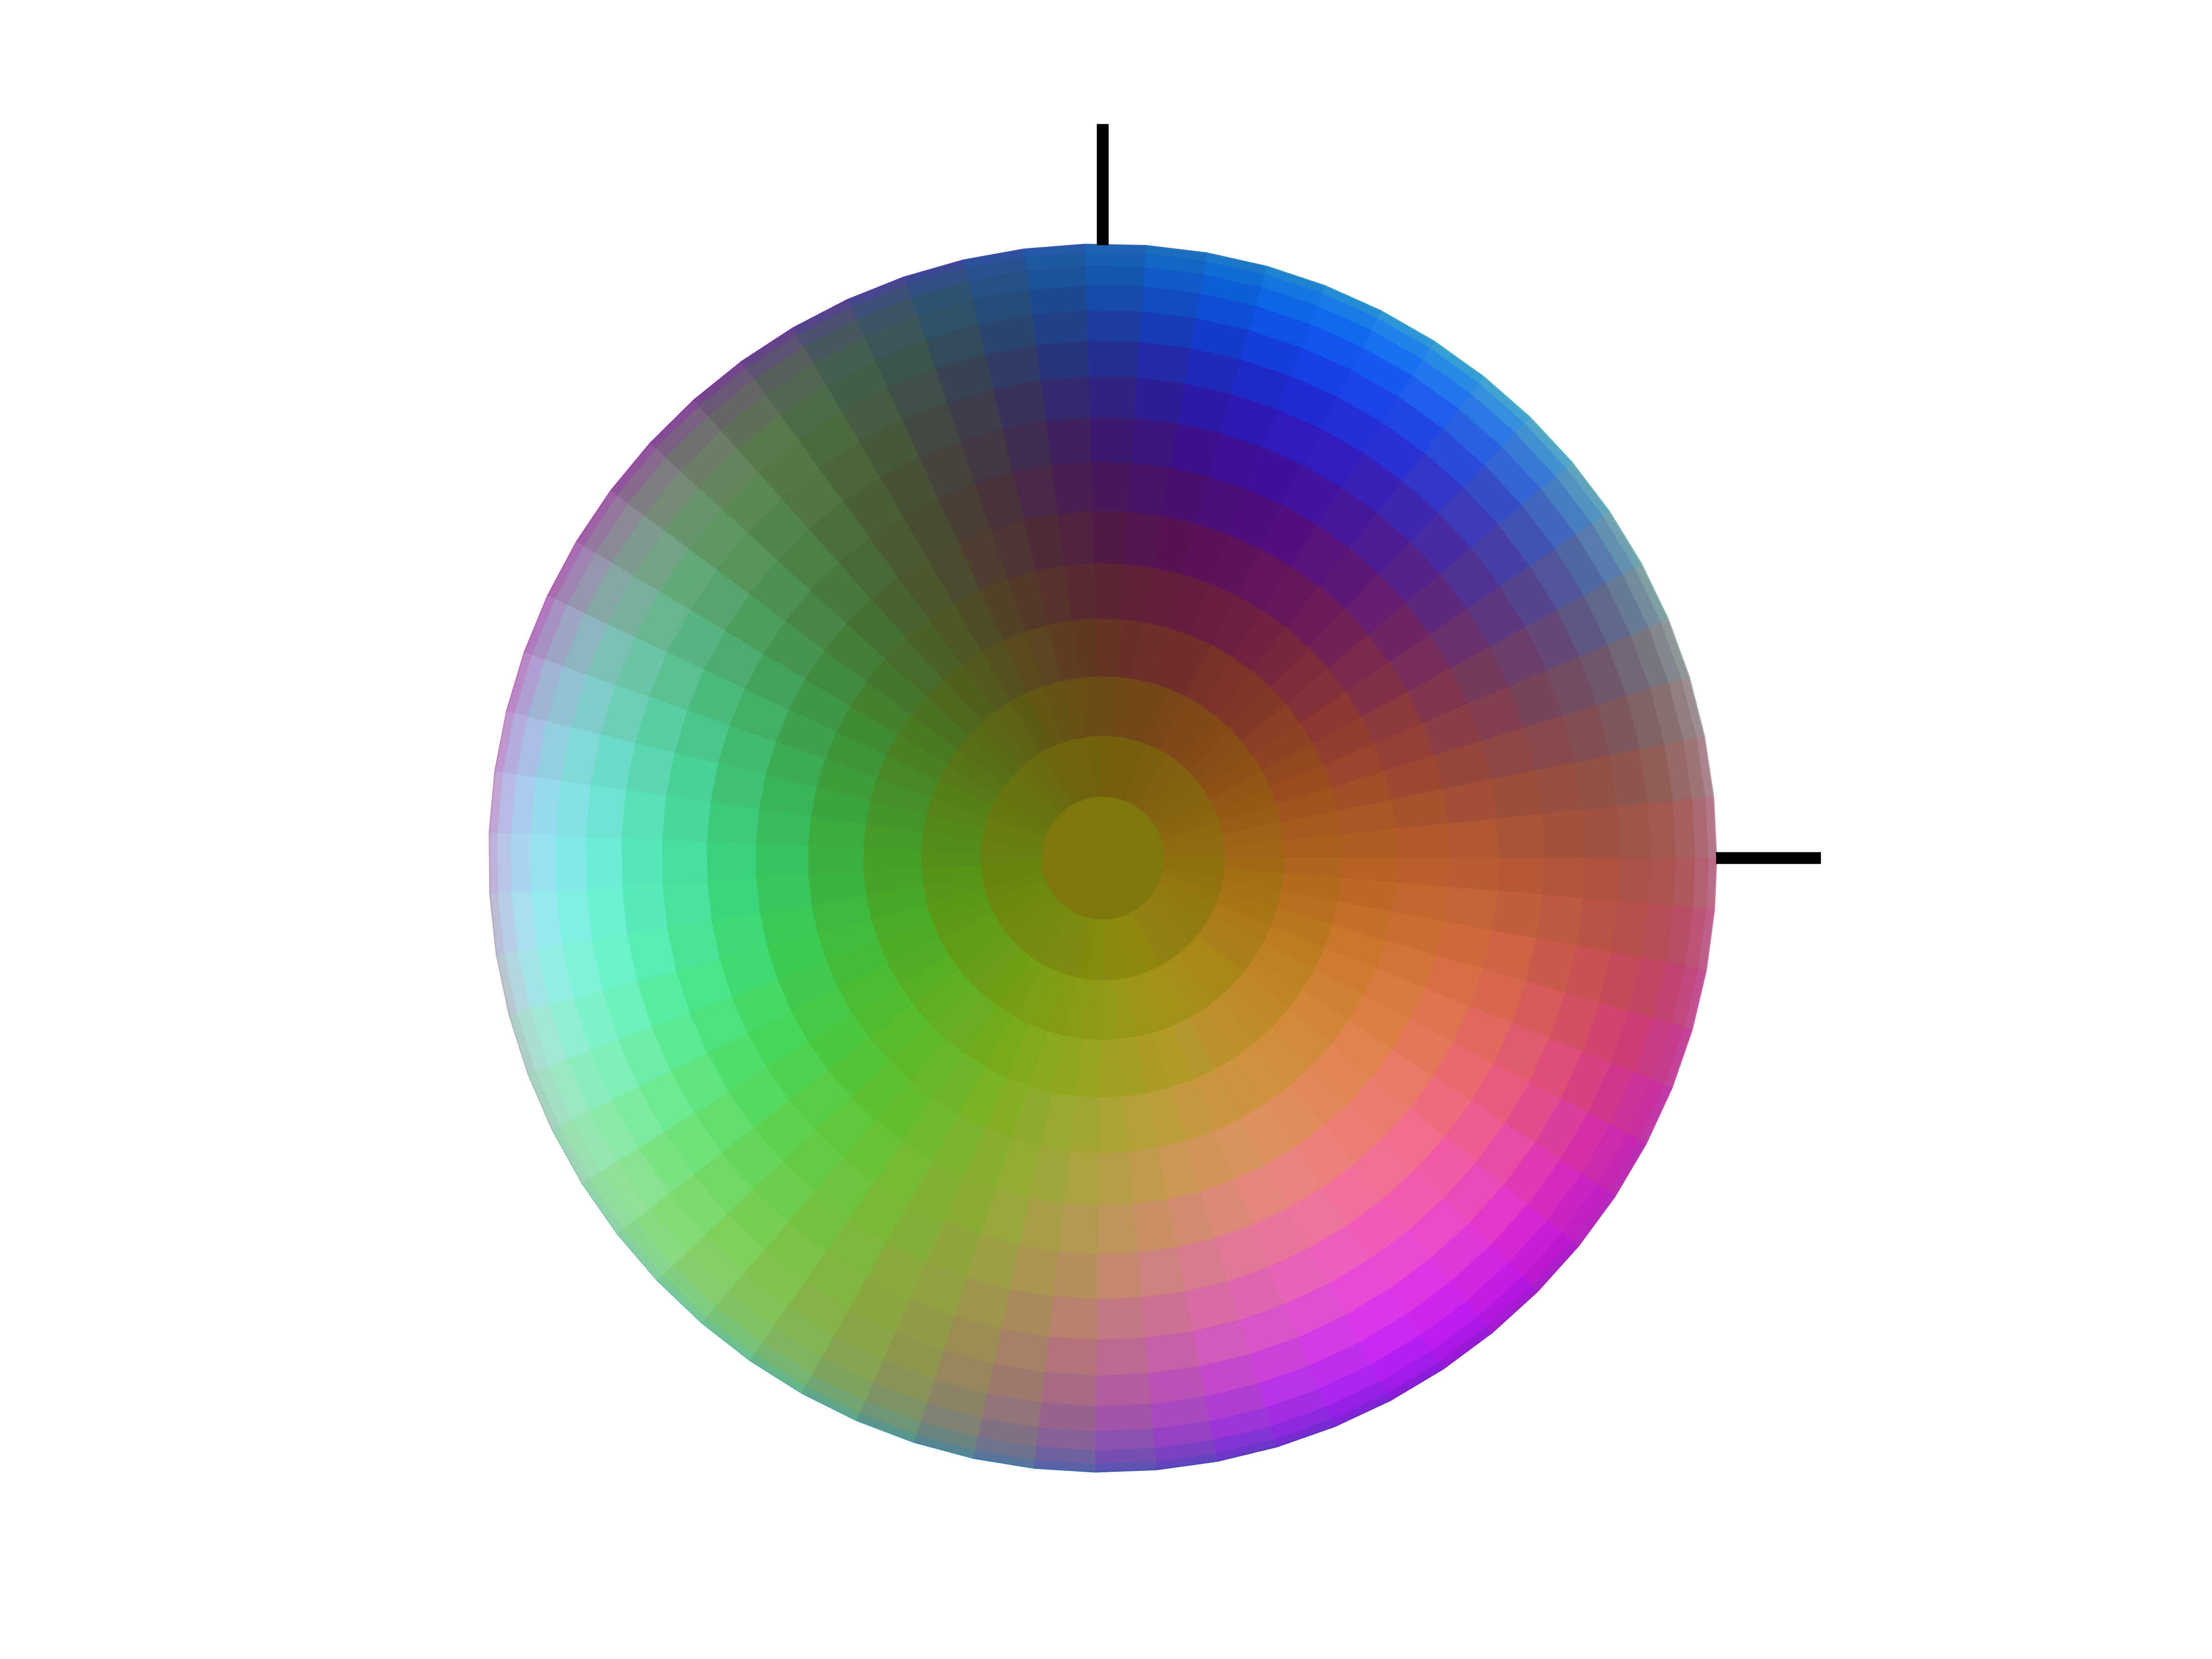
\includegraphics[width=0.3\textwidth]{boys_zIn_yRight}
		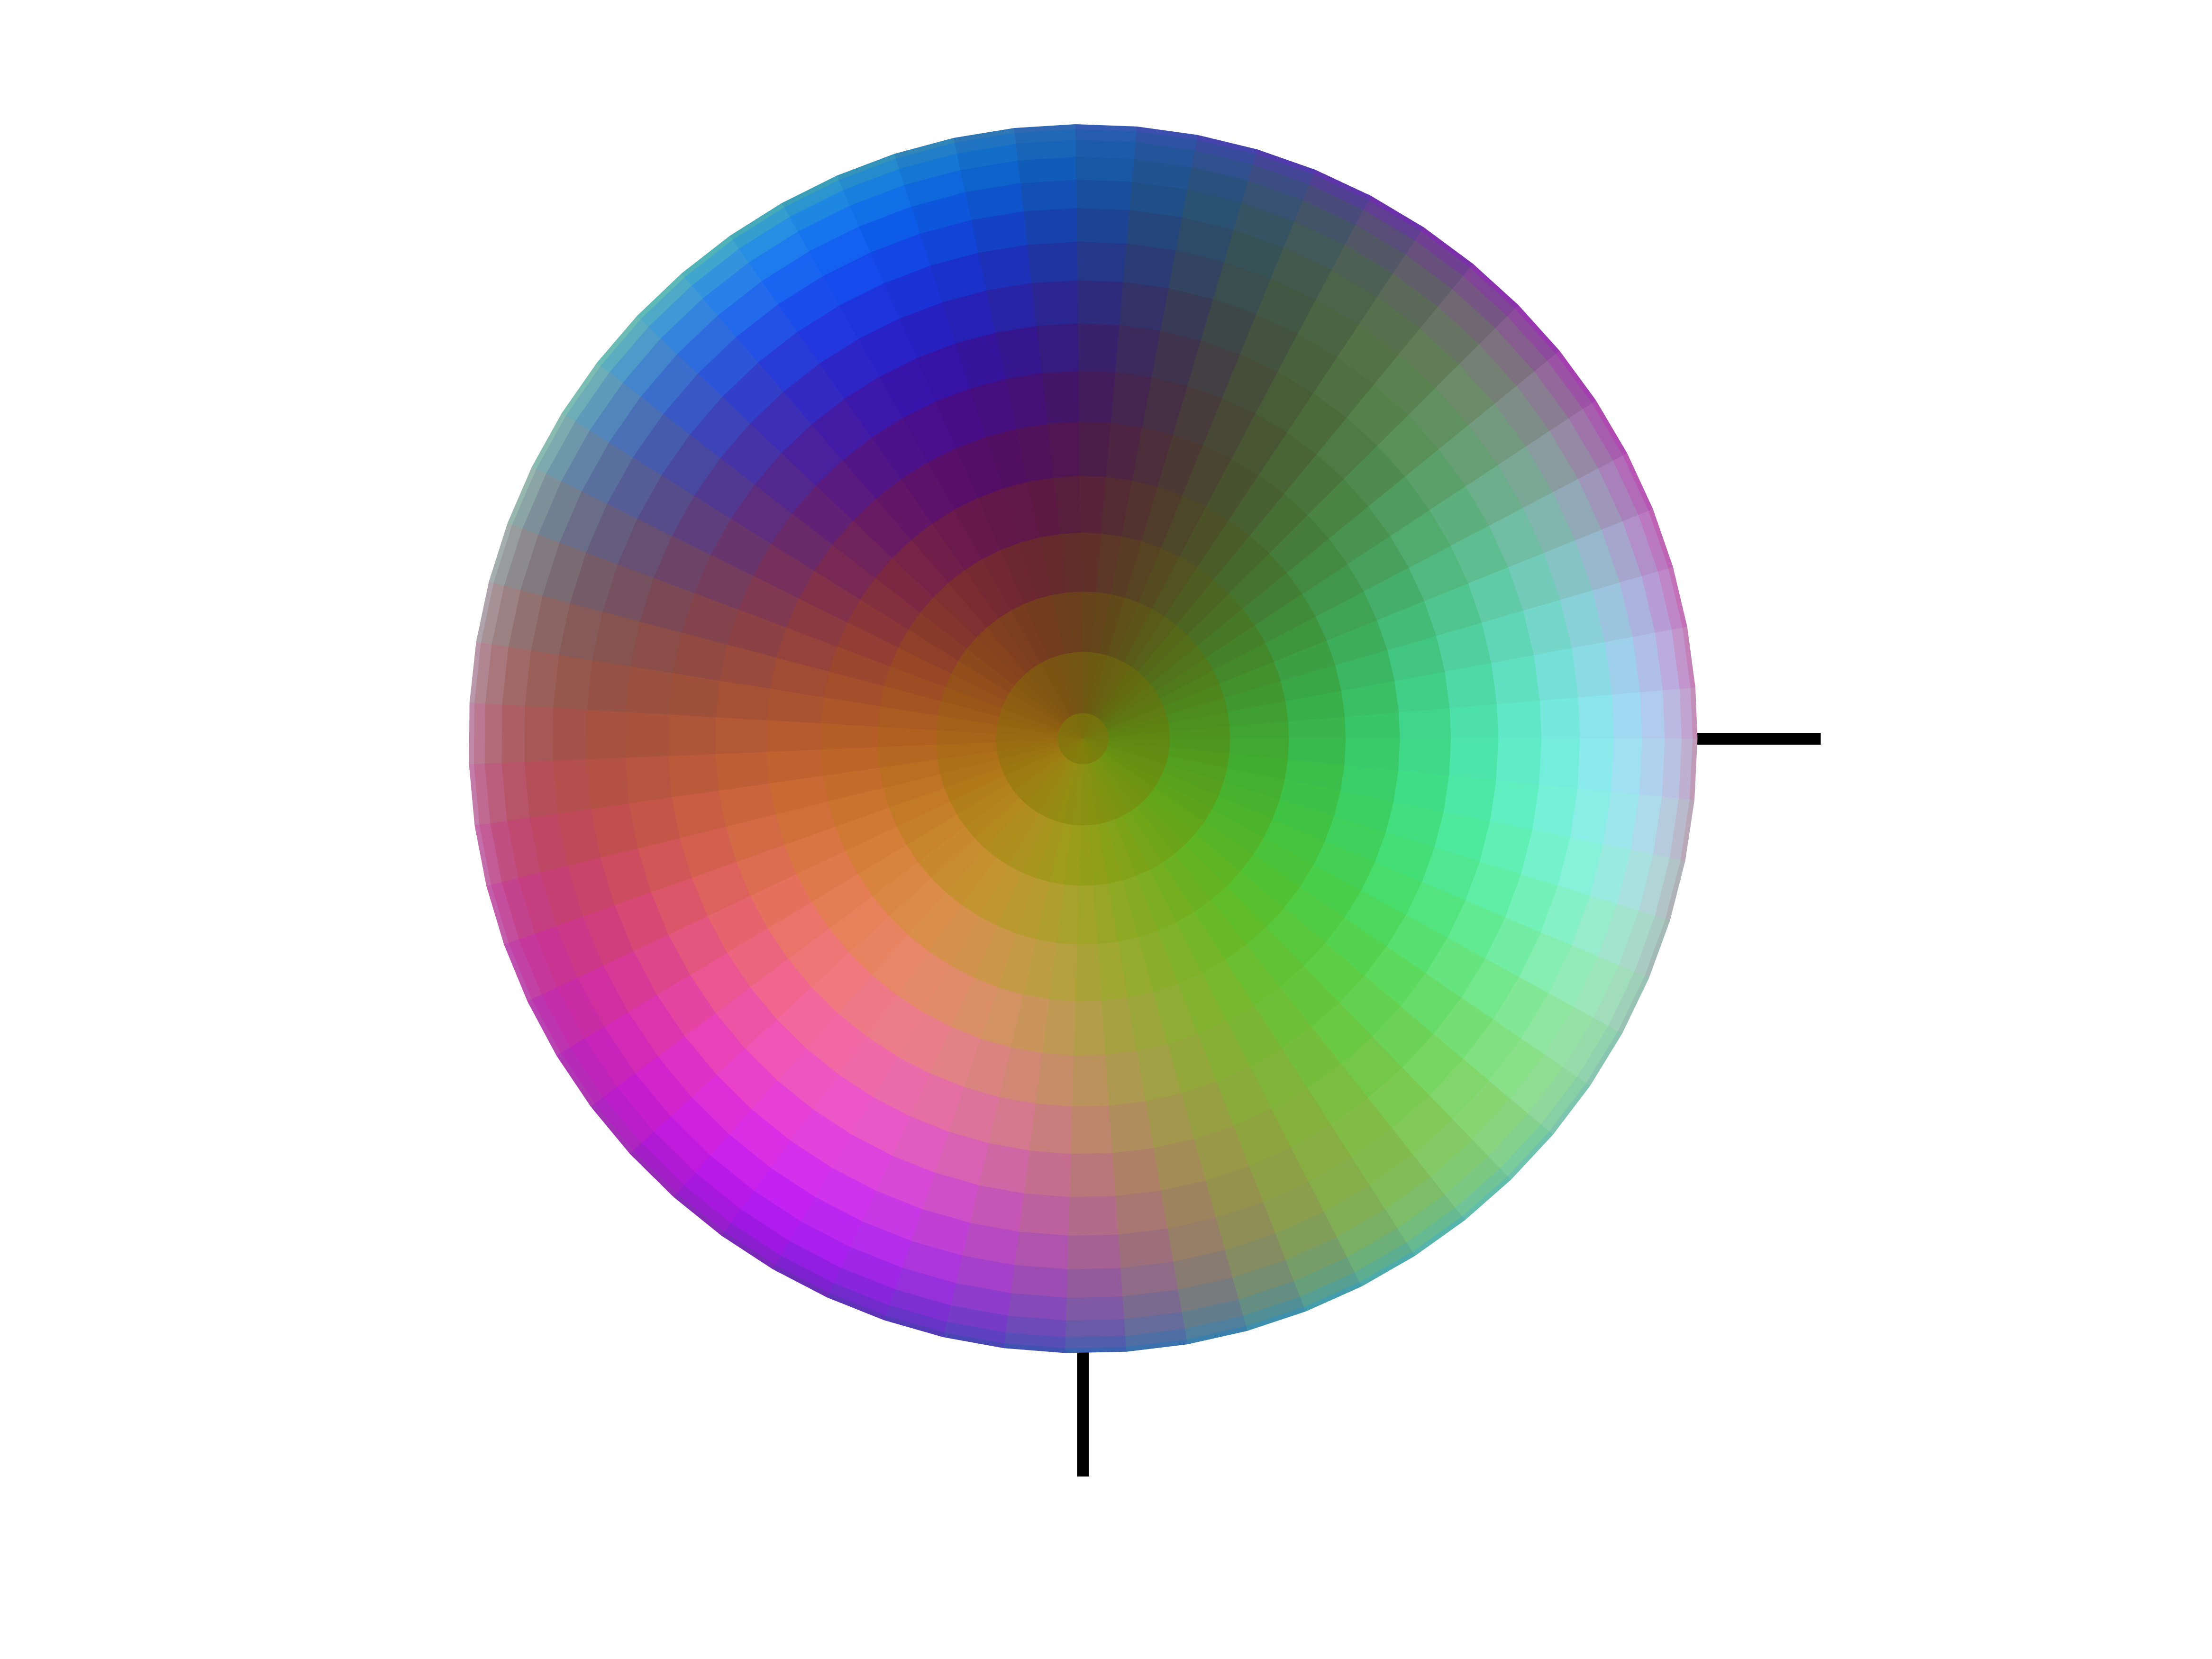
\includegraphics[width=0.3\textwidth]{boys_zOut_yRight}
		\caption{Boy's surface method, colored sphere.}
	\end{figure}



\end{document}

